\documentclass[10pt,a4paper]{article}
\usepackage{fontspec,polyglossia}
\setmainlanguage{russian}
\setmainfont{Times New Roman}
\usepackage{amsmath,amssymb,booktabs,tabularx,graphicx}
\usepackage[margin=17mm]{geometry}
\usepackage[hidelinks]{hyperref}
\usepackage{titlesec}
\titleformat{\section}{\large\bfseries}{}{0pt}{}
\titlespacing*{\section}{0pt}{8pt}{4pt}
\setlength{\parindent}{0pt}
\setlength{\parskip}{4pt}
\setlength{\emergencystretch}{3em}
\begin{document}
{\Large\bfseries Neural collapse и MG при обучении классификатора изображений}\par\medskip

29 сентября 2026. Выполненный CPU-пилот на CIFAR-10.

\textbf{Результат:} упрощение представлений независимо подтверждено в трёх запусках, но MG истории loss не стал надёжным индикатором этого упрощения. Преимущество над простыми альтернативами не обнаружено. Этот эксперимент пока не подходит в качестве положительного примера для статьи.

\section*{Зачем этот эксперимент}

Проверяем прикладную гипотезу: можно ли по одному числу на шаг обучения дешёво следить за формированием более простой геометрии признаков. Не требуем восстановления точного числа активных компонент. Neural collapse [1] даёт независимый ориентир: признаки изображений одного класса сближаются относительно расстояния между классами; расположение центров становится регулярнее.

\section*{Кто учится, на чём и как}

Обучается классификатор десяти классов CIFAR-10 [2], который получает RGB-изображение 32\ensuremath{\times}32 и предсказывает класс. Это реальная задача распознавания, но уменьшенный эксперимент: 2 000 изображений для обучения и 1 000 из официальной тестовой части, строго по 200 и 100 на класс. Разбиение фиксировано, seed 20260929; подбор по качеству или MG не проводился. Дополнительные тестовые наблюдения не участвуют в градиентах.

Модель: небольшой ResNet с 78 032 параметрами. Начальная свёртка 3\ensuremath{\times}3, ширина 16; три residual-блока по две свёртки с ширинами 16/32/64, downsampling во втором и третьем блоках; BatchNorm, ReLU, global average pooling; линейная голова без bias из 64 признаков в 10 классов. Все веса обучаются с нуля.

Cross-entropy, SGD с momentum 0,9, weight decay 0,0005, \textbf{постоянный} learning rate 0,03. Batch 64, независимая равномерная выборка с возвращением на каждом шаге. 4 096 шагов, примерно 131 эквивалент прохода по подвыборке; seeds 0/1/2. Изображения нормированы, без аугментаций, без искусственного ограничения ранга и без штрафа за collapse. Нормировка RGB: mean=(0,4914; 0,4822; 0,4465), std=(0,2470; 0,2435; 0,2616).

\section*{Что получает MG и что измеряется независимо}

Время --- шаг SGD. MG анализирует три отдельных ряда: loss случайного обучающего batch до обновления; loss фиксированных 100 обучающих изображений после обновления; loss фиксированных 100 тестовых изображений. Оба фиксированных набора сбалансированы. Их обработка идёт в eval-режиме и не изменяет BatchNorm.

Каждые 128 шагов извлекаем все 64-мерные признаки 2 000 обучающих изображений. Пусть h\_i --- признак, y\_i --- класс, \ensuremath{\mu}\_c --- средний признак класса, \ensuremath{\mu} --- среднее десяти центров; K=10 и n=2000. Вычисляем:

\[
\Sigma_W=\frac1n\sum_i(h_i-\mu_{y_i})(h_i-\mu_{y_i})^\top,\quad
\Sigma_B=\frac1K\sum_c(\mu_c-\mu)(\mu_c-\mu)^\top,\quad
\mathrm{NC1}=\frac1K\operatorname{tr}(\Sigma_W\Sigma_B^\dagger).
\]

Меньший NC1 означает меньший относительный внутриклассовый разброс в данной метрике. Дополнительно сохранено tr(\ensuremath{\Sigma}\_W)/tr(\ensuremath{\Sigma}\_B). NC2 --- нормированное расстояние матрицы косинусов центрированных центров до правильного симплекса; NC3 --- расстояние между нормированными матрицами весов головы и центров; NC4 --- доля разногласий классификатора и ближайшего центра. NC1--NC3 лучше при уменьшении, NC4 лучше при приближении к нулю. Полные определения и допуски --- в коде и PROTOCOL.md.

\newpage

\section*{Упрощение действительно произошло}

\begin{center}\small
\begin{tabularx}{\linewidth}{>{\raggedright\arraybackslash}X>{\raggedright\arraybackslash}X>{\raggedright\arraybackslash}X>{\raggedright\arraybackslash}X>{\raggedright\arraybackslash}X}
\toprule
Seed & Первый шаг с train accuracy 100\% & NC1 на этом шаге \ensuremath{\to} в конце & NC2 на этом шаге \ensuremath{\to} в конце & Test accuracy в конце \\
\midrule
0 & 1152 & 0,626 \ensuremath{\to} 0,237 & 0,866 \ensuremath{\to} 0,624 & 51,7\% \\
1 & 1280 & 0,586 \ensuremath{\to} 0,364 & 0,850 \ensuremath{\to} 0,712 & 51,5\% \\
2 & 1280 & 0,537 \ensuremath{\to} 0,250 & 0,875 \ensuremath{\to} 0,724 & 50,5\% \\
\bottomrule\end{tabularx}\end{center}

После первого достижения нулевой тренировочной ошибки NC1 дополнительно уменьшился на 38--62\%. К концу NC4=0 во всех трёх запусках, NC3=0,309--0,320. Это подтверждает \textbf{тенденцию к neural collapse}, но не достижение идеального симплекса: NC2 остаётся заметно выше нуля. Улучшение обобщения не продемонстрировано: тестовая точность находится около 51\%.

\begin{center}
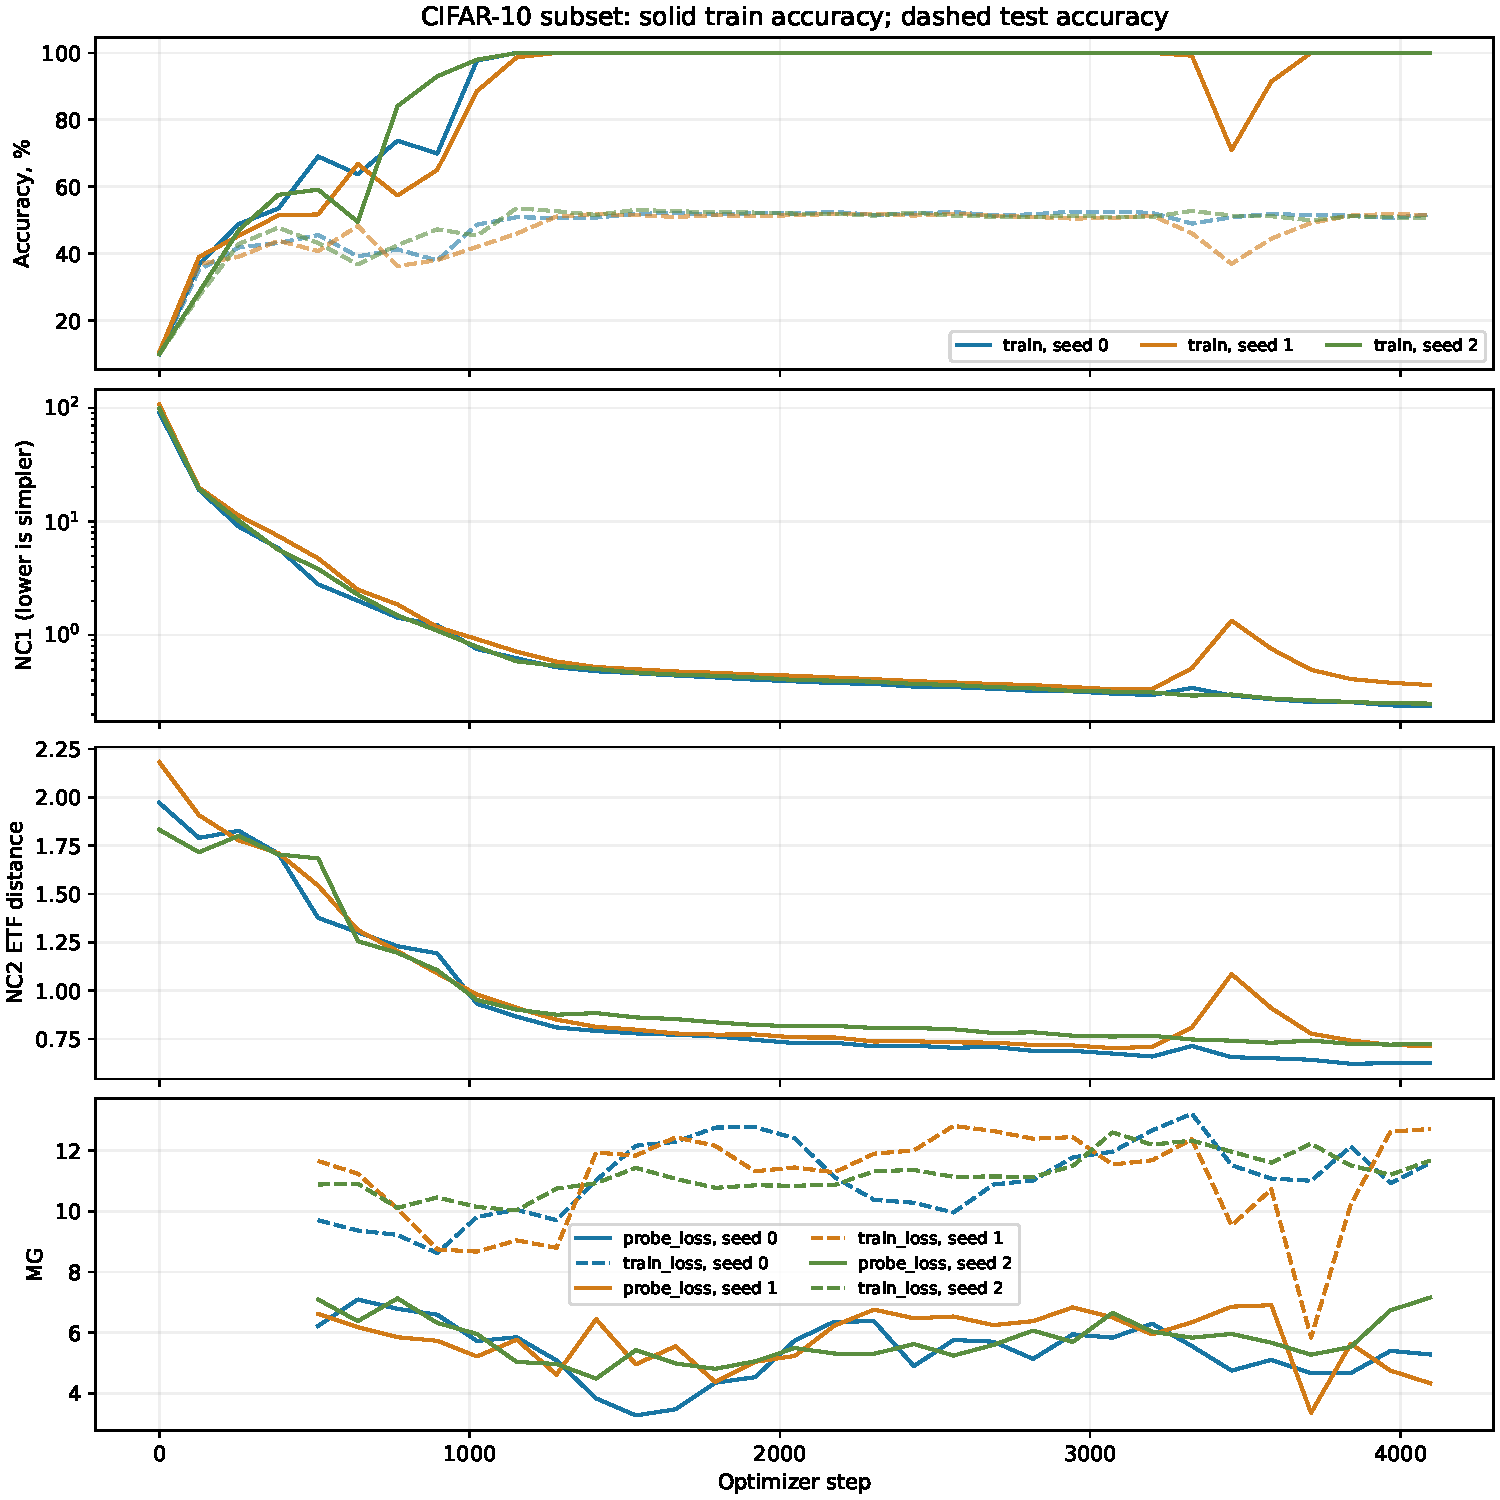
\includegraphics[width=\linewidth,height=.49\textheight,keepaspectratio]{results/training_and_mg.pdf}
\end{center}

Сплошные линии точности --- train, пунктир --- test. На нижней панели сплошные линии MG относятся к фиксированному обучающему набору, пунктирные --- к случайным batch. У seed 1 на шагах 3328--3584 есть временный срыв train accuracy и геометрии; он сохранён в анализе, а не удалён. Поэтому период после первого нуля ошибки нельзя целиком считать устойчивой терминальной фазой.

\newpage

\section*{MG не отслеживает это упрощение надёжно}

Основная конфигурация зафиксирована до анализа: W=512 шагов, E=20, \ensuremath{\tau}=1, k=20 соседей, исключение Theiler=39 шагов, расчёт раз в 128 шагов. Используется исходный pooled MG из проекта. Для проверки устойчивости считаем E=40 при тех же \ensuremath{\tau} и исключении. Ранний интервал --- окна с концами на шагах 512--1024; поздний --- последние 1024 шага. Таблица: поздняя медиана, делённая на раннюю.

\begin{center}\small
\begin{tabularx}{\linewidth}{>{\raggedright\arraybackslash}X>{\raggedright\arraybackslash}X>{\raggedright\arraybackslash}X>{\raggedright\arraybackslash}X}
\toprule
Запуск & MG фиксированного train loss & MG фиксированного test loss & MG batch loss \\
\midrule
Обучение, seed 0 & 0,788 & 0,735 & 1,233 \\
Обучение, seed 1 & 0,989 & 0,949 & 1,111 \\
Обучение, seed 2 & 0,924 & 0,768 & 1,130 \\
Замороженные признаки, seed 0 & 0,815 & 0,592 & 1,061 \\
\bottomrule\end{tabularx}\end{center}

В обучаемых запусках MG фиксированного train loss падает в среднем на 9,9\%, но корреляции с NC1 равны 0,259; \ensuremath{-}0,024; \ensuremath{-}0,158. Среднее того же loss согласуется с NC1 сильнее: 0,741; 0,862; 0,942. У MG тестового loss корреляции 0,845; 0,110; 0,481, но корреляции первых разностей всего 0,008; 0,149; 0,018. Общего тренда недостаточно для утверждения, что MG следит за изменениями геометрии.

\textbf{Главный отрицательный контроль:} обучаем только линейную голову, замораживая признаки и статистики BatchNorm. Аудит сохранённых признаков даёт точное нулевое изменение. NC1=91,183 и NC2=1,972 постоянны, но MG фиксированного train loss уменьшается на 18,5\%, а test loss --- на 40,8\%. Это не исключает изменений динамики головы; это показывает неспецифичность MG к neural collapse признаков.

\begin{center}
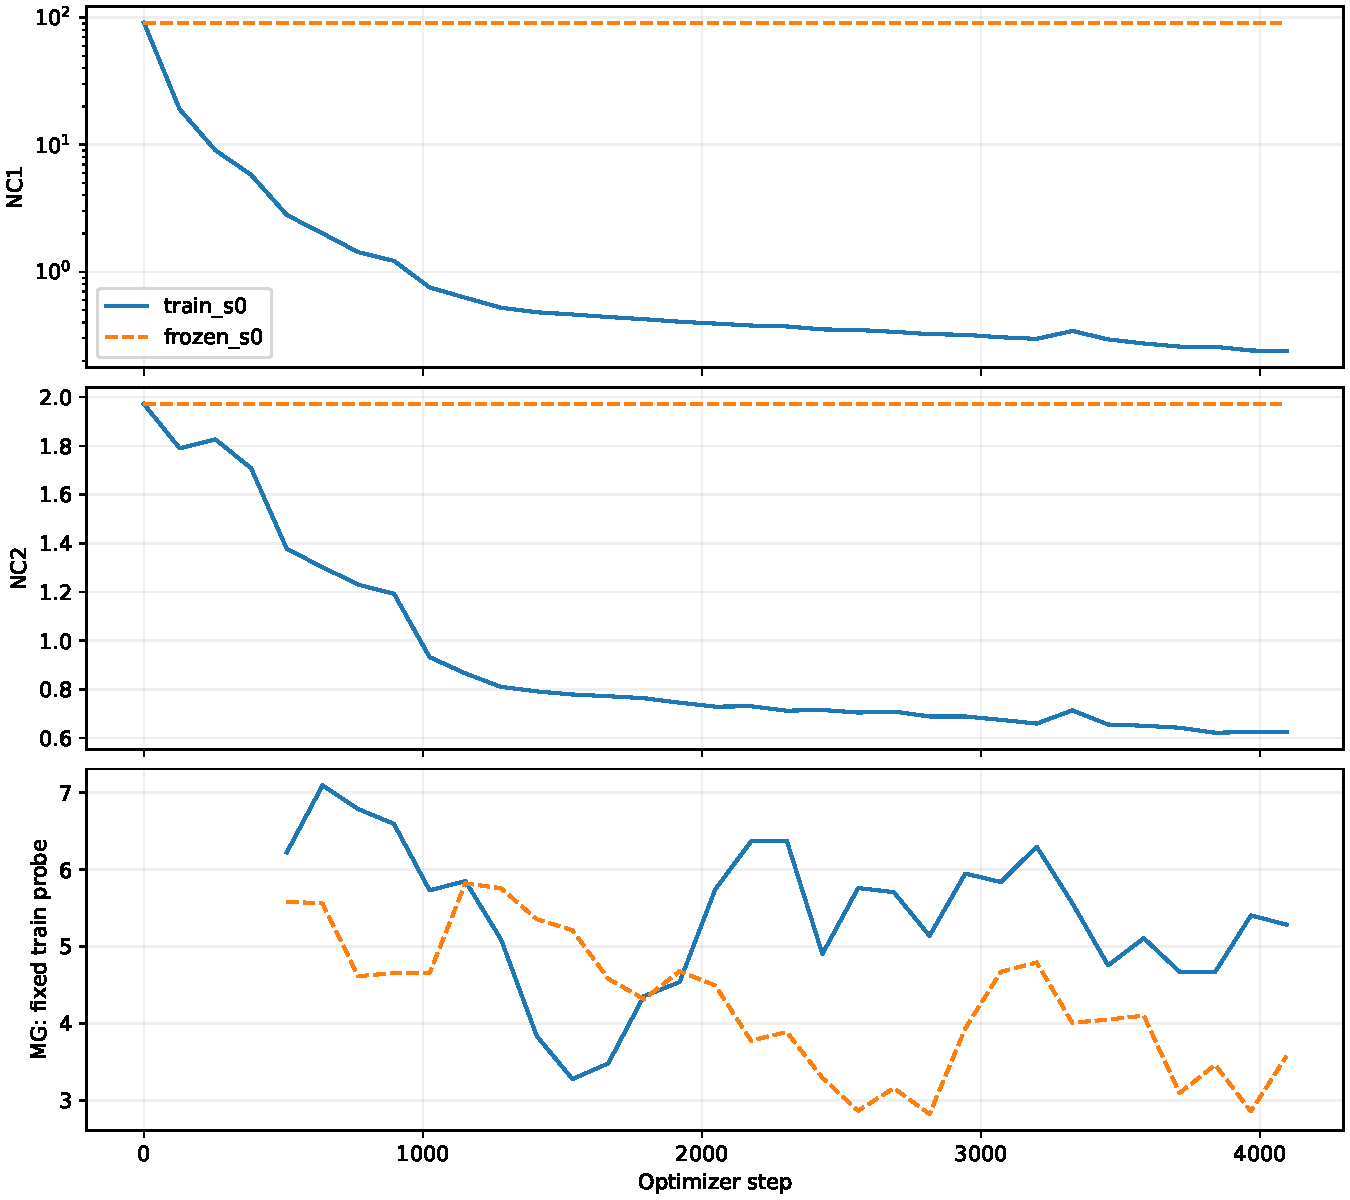
\includegraphics[width=\linewidth,height=.33\textheight,keepaspectratio]{results/frozen_control.pdf}
\end{center}

Проверки W=256/1024 и \ensuremath{\tau}=4 не устранили проблему: например, при W=1024 поздний/ранний MG train-probe равен 0,973; 1,143; 1,001. В этом варианте раннее окно только одно, поэтому сравнение описательное. Для основного варианта позднее MG(40)/MG(20)=1,34--1,50; численно вырожденных окон нет. Это не даёт гарантии абсолютной размерностной интерпретации.

\newpage

\section*{Стоимость и сильный дешёвый конкурент}

Измерения проведены последовательно на CPU Intel Core i5-12500H; PyTorch 2.10.0+cpu, NumPy 2.4.3. Обучение и извлечение признаков: 8 потоков PyTorch, BLAS=1; MG и его соседи: 1 поток. GPU не использовался. Для MG сохранены три повтора на основное окно; для итогового контроля времени --- семь вызовов, первые два исключены. Все числа ниже округлены.

\begin{center}\small
\begin{tabularx}{\linewidth}{>{\raggedright\arraybackslash}X>{\raggedright\arraybackslash}X}
\toprule
Измерение & Время \\
\midrule
MG уже записанного train-probe loss, одно окно & 9--10 мс \\
MG с E40 и диагностикой, 29 окон & 0,61--0,66 с \\
Полная NC-геометрия 2000 изображений, один checkpoint & 257 мс \\
NC-геометрия 100 изображений, один checkpoint & 13 мс \\
Простые статистики одного scalar-окна & 0,2--0,5 мс \\
\bottomrule\end{tabularx}\end{center}

Чистый MG примерно в 26--29 раз быстрее полной проверки NC на сопоставленном checkpoint; с диагностикой --- в 11--12 раз. Но для его фиксированного loss нужен forward на каждом из 4 096 шагов. Если такого лога ещё нет, сбор добавляет примерно 49--52 с; весь MG-monitor занимает около 50--53 с против 7,4--7,8 с для 29 полных проверок NC. Это \textbf{оценка полной стоимости} по повторным замерам одиночного probe-forward; фактически в обучении два probe вычислялись совместно, их измеренное время сохранено отдельно. Сам training loss дополнительного forward не требует, но его MG растёт, а не следует снижению NC1.

Ещё важнее контроль по маленькой выборке: NC1 по 100 изображениям коррелирует с полной оценкой на уровне 0,988--0,999. Его абсолютные значения смещены, однако динамика воспроизводится хорошо. Такой контроль достаточно считать только на 29 checkpoint: около 0,38 с вместе с извлечением признаков. В данной задаче он практичнее непрерывного probe-log и специфичнее MG. Победа только над полной выборкой была бы неполным сравнением.

\section*{Что следует для статьи}

\textbf{Положительный факт:} на реальных изображениях независимо наблюдается упрощение обучаемых представлений. \textbf{Проверяемая гипотеза о MG не получила достаточной поддержки:} направление и сила отклика зависят от наблюдаемого loss и окна, похожее падение есть при неизменной геометрии, а простые альтернативы сильнее. Поэтому этот запуск нельзя добавлять как подтверждение «MG надёжно и дешевле отслеживает neural collapse».

Это не опровержение MG как анализатора других видов динамики. Neural collapse характеризует распределение признаков разных изображений в один момент; MG здесь характеризует временную последовательность loss. Связь этих объектов оказалась слабой. Следующий осмысленный шаг --- отдельно проверить наблюдение, ближе связанное с представлениями, либо другую прикладную задачу; настройка окна по этим же результатам не будет независимой валидацией.

Ограничения: одна небольшая архитектура, 2 000 обучающих изображений, три инициализации на одном разбиении; только один frozen-control. CIFAR-100 и полный CIFAR-10 не запускались. Нет независимой проверки выбранных гиперпараметров на новых seeds. Перекрывающиеся окна не считаются независимыми наблюдениями; корреляции описательные, статистическая значимость не заявляется. Полную идентификацию active dimension целью не ставили.

\section*{Воспроизводимость и проверка}

Исходники и результаты находятся в research\_neural\_collapse. PROTOCOL.md фиксирует постановку; run.py обучает, analyze.py строит MG и таблицы, benchmark.py проверяет время, build\_report.py собирает отчёт. В results сохранены логи всех 4\ensuremath{\times}4096 шагов, признаки всех checkpoint, финальные веса, индексы изображений и SHA-256 исходных batch-файлов. Для повторения команд см. README.md.

Проверены нулевые NC-метрики для идеального симплекса, инвариантность к общему масштабу и вращению, повторный расчёт финальной геометрии из сохранённых признаков, неизменность признаков frozen-control. Результаты аудита --- results/audit.json. Статья и её шесть PDF не изменялись.

[1] Papyan V., Han X. Y., Donoho D. L. Prevalence of Neural Collapse during the Terminal Phase of Deep Learning Training. PNAS, 2020. DOI: 10.1073/pnas.2015509117.

[2] Krizhevsky A. Learning Multiple Layers of Features from Tiny Images, 2009. Официальные CIFAR-10 Python batches, University of Toronto.
\end{document}
